\subsection{Installation de l'application}
Avant de présenter cette application, nous allons détailler la manière d'installer cette application sur un poste. On supposera dans cette démarche que le poste en question est équipé de MySQL et d'un serveur WAMP/MAMP.

\subsubsection{Installation de la base de données}
Tous les codes relatifs à la base de données sont présents dans le fichier \texttt{telephonie/database} de l'archive qui vous a été remise. Ce répertoire contient alors plusieurs types de fichiers :
\begin{itemize}
  \itemperso{\texttt{DB.php}}Ce fichier correspond à la classe PHP développée pour réaliser la connexion à la base de données et l'exécution des requêtes/procédures vers cette base de données. Cette classe sera détaillée dans la Section~\ref{sec:elaboration-bdd}.
  \itemperso{\texttt{create\_table.sql}}Les requêtes SQL permettant de recréer la structure des tables SQL.
  \itemperso{\texttt{.*\_procedures.sql}}Ces fichiers contiennent pas groupes thématiques (utilisateurs, téléphones, achats,...) les procédures à stocker dans la base de données, ainsi que des instruction pour remplir les différentes tables de la base de données.
  \itemperso{\texttt{update\_DB.sh}}Ce script permet de lancer \og automatiquement\fg{} l'installation de la base de données à partir des procédures stockées et de l'extraction de la structure de la base de données proposée dans le fichier \texttt{create\_table.sql}.
\end{itemize}

Ainsi, pour installer la base de données, seule deux étapes sont nécessaires :
\begin{itemize}
  \itemperso{Première étape}Ouvrir le fichier \texttt{update\_DB.sh} et adapter les informations de connexion à la base de données en fonction de votre propre installation (nom de la base, mot de passe,...). La ligne à considérer est la suivante (ici, pas de mot de passe pour \texttt{root} par exemple) :
\begin{lstlisting}
  mysql --default-character-set=utf8 -h localhost -u root --password='' telephonie < temp.sql
\end{lstlisting}
  \itemperso{Seconde étape}Lancer ce même script (\texttt{update\_DB.sh}) une fois que les informations remplies correspondent à votre configuration. Normalement, la base de données devrait se remplir automatiquement, en créant la structure des tables, en enregistrant les procédures qui doivent l'être et en se remplissant avec un ensemble de données test. Si toute fois l'installation a échoué, veuillez importer directement dans votre base de données le fichier \texttt{temp.sql} qui vient d'être généré et qui contient toutes les commandes nécessaires à l'import de la base.
\end{itemize}

\subsubsection{Installation du code source}
\subParagraphe{Extraction de l'archive}Une fois l'installation de la base de données réalisée, il est alors nécessaire d'installer le code source de l'application sur votre poste afin de pouvoir tester l'interface développée pour ce projet.

Pour se faire, il vous faudra extraire le dossier \texttt{telephonie} de l'archive qui a été remise dans le dossier \texttt{www} correspondant à votre installation locale de WAMP/MAMP. Par exemple pour un poste équipé de Windows, ce dossier se situe généralement à \texttt{C:\textbackslash wamp\textbackslash www}.

\subParagraphe{Téléchargement d'un module}Le code fourni est cependant incomplet, et ne permettra pas de gérer la génération du PDF de facture pour un client. En effet, nous avons pour cela utilisé une bibliothèque supplémentaire. Cependant, le code de cette dernière faisant 13Mo, nous n'avons pu l'inclure à cette archive, sans quoi nous ne pouvions plus la poster sur \texttt{pedagogie} (limite élève à $7,5$Mo).

Ainsi, nous vous proposons de récupérer le contenu de cette bibliothèque directement sur le GitHub du projet :
\begin{center}
  \texttt{https://github.com/stity/projet\_sql/tree/master/vue}
\end{center}
Le fichier à récupérer est le fichier \texttt{fop}, à inclure dans le dossier \texttt{vue} de l'application.

Il est à noter que ce module sert uniquement pour la génération de PDF, et n'est pas utilisé pour le reste de la plateforme...

\subsubsection{Test de bon fonctionnement}
Une fois le code installé et la base de données préparée, vous êtes désormais prêt pour tester l'application! Pour cela, lancer votre serveur WAMP/MAMP, et rendez vous à l'adresse suivante :
\begin{center}
  \url{http://localhost/telephonie/index.php}
\end{center}
Si vous voyez l'écran de la Figure~\ref{fig:hello-world} s'afficher, c'est que la procédure d'installation a correctement marchée (à minima, vu qu'on ne teste pas ici toute la base de données!).

\begin{figure}[ht]
  \centering
  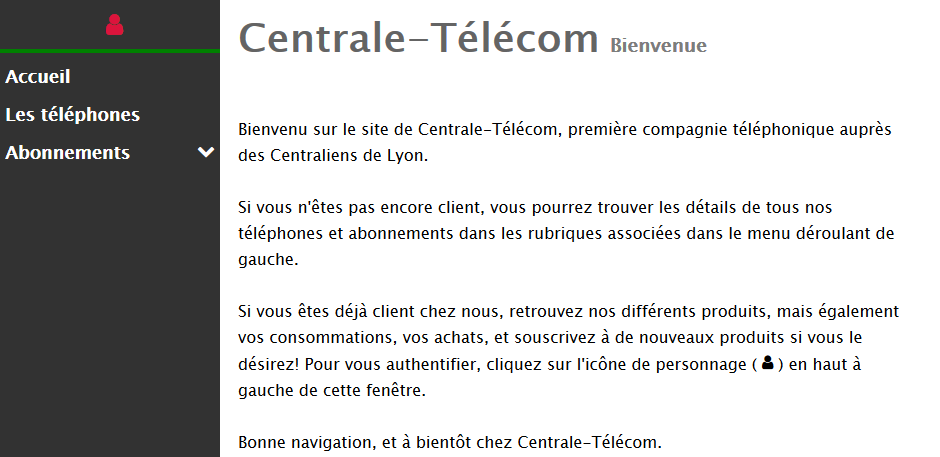
\includegraphics[width=.5\textwidth]{images/Travail_realise/hello-world}
  \caption{\'Ecran d'accueil de l'application}
  \label{fig:hello-world}
\end{figure}

%%% Local Variables:
%%% mode: latex
%%% TeX-master: "../../Rapport_BDD"
%%% End:
